\documentclass{beamer}
\usetheme{ucl}

\newcommand\hmmax{0}
\newcommand\bmmax{0}

\usepackage{graphicx}%
\usepackage{multirow}%
\usepackage{amsmath,amssymb,amsfonts}%
%\usepackage{amsthm}%
\usepackage{stmaryrd}
\usepackage{mathrsfs}%
\usepackage[title]{appendix}%
\usepackage{xcolor}%
\usepackage{textcomp}%
\usepackage{manyfoot}%
\usepackage{booktabs}%
\usepackage{algorithm}%
\usepackage{algorithmicx}%
\usepackage{algpseudocode}%
\usepackage{listings}%
\usepackage{orcidlink}
\usepackage{comment}
%%%%
\usepackage{mathtools}  % For cases
%\usepackage{thm-restate}
%\usepackage{mathrsfs}
%\usepackage[inline]{enumitem} %For enum*

\usepackage{mathbbol}
%\usepackage{tikz-cd} % For tikz art
%\usepackage{tikzit}
%\usepackage{ebproof}
\usepackage{bussproofs}
\usepackage{proof}


%%%%%%%%%%%%%%%%%%%%%%%%%%%%%%%%%%%%%%%%%%%%%%%%%%%%%%
%%%%%%%%%%%%%% Define the new environments here;
%\newenvironment{qparts}{\begin{enumerate}[{(}a{)}]}{\end{enumerate}}
% \def\endproofmark{$\Box$}
%\renewenvironment{proof}{\par{\bf Proof}:}{\hfill$\blacksquare$}

\newtheorem{defn}[theorem]{Definition}

\newtheorem{question}[theorem]{Question}
\newtheorem{remark}[theorem]{Remark}
\newtheorem{construction}[theorem]{Construction}
\newtheorem{observation}[theorem]{Observation}

%Make font sans-serif
\renewcommand{\familydefault}{\sfdefault}

%%%%%% Define commands here;

% Basic logic notation.
%\newcommand{\seq}{\triangleright}
\newcommand{\seq}{\Rightarrow }
\newcommand{\sequent}[2]{{#1} \seq {#2}}
\newcommand{\thmSequent}[2]{{#1} \vdash {#2}}

%%%%%%%%%%%%%%%%%%%%%%%%%%%%%%%%%%%%%%%%%
%       BeS
%%%%%%%%%%%%%%%%%%%%%%%%%%%%%%%%%%%%%%%%%
\newcommand{\base}[1]{\mathscr{#1}}
\newcommand{\baseB}{\base{B}}
\newcommand{\baseC}{\base{C}}
\newcommand{\baseD}{\base{D}}
\newcommand{\baseE}{\base{E}}
\newcommand{\baseF}{\base{F}}
\newcommand{\baseG}{\base{G}}
\newcommand{\baseH}{\base{H}}
\newcommand{\baseX}{\base{X}}
\newcommand{\baseY}{\base{Y}}
\newcommand{\baseZ}{\base{Z}}
\newcommand{\baseILL}{\base{N}}
\newcommand{\emptybase}{\varnothing}
\newcommand{\basis}[1]{\mathfrak{#1}}
% \newcommand{\at}[1]{\mathrm{#1}}
\newcommand{\at}[1]{{#1}}
\newcommand{\At}{\mathbb{A}}

%\newcommand{\baseGeq}{\succeq}
%\newcommand{\baseLeq}{\preceq}
\newcommand{\baseGeq}{\supseteq}
\newcommand{\baseLeq}{\subseteq}

\newcommand{\suppTor}[1]{\Vdash_{\!\!#1}}
% \newcommand{\supp}[1]{\Vdash_{\!\!#1}}
% \newcommand{\suppNew}[1]{\vDash_{\!#1}}
\newcommand{\suppNew}[1]{\Vdash^{*}_{\!#1}}
\newcommand{\entails}{\Vdash}
%\newcommand{\proves}[1]{\vdash_{\!\!#1}}
\newcommand{\proves}{\vdash}
\newcommand{\plus}{+}
\newcommand{\system}[1]{\mathsf{#1}}
\newcommand{\Atoms}{\set{A}}
\newcommand{\Formulas}{\set{F}}
\newcommand{\Bunches}{\set{B}}
\newcommand{\set}[1]{\mathbb{#1}}


%%%% ILL
%%%% ILL
\newcommand{\IPL}{IPL}
\newcommand{\IMLL}{IMLL}
\newcommand{\IMALL}{IMALL}
\newcommand{\ILL}{ILL}
%\newcommand{\provesIMALL}{\vdash_{\mathrm{IMALL}}}
%\newcommand{\provesILL}{\vdash_{\mathrm{ILL}}}
\newcommand{\provesILL}{\vdash}
\newcommand{\multiset}{\mathcal{M}}
\newcommand{\fmultiset}{\mathcal{M}_{\!{f}}}
\newcommand{\emptymultiset}{\varnothing}
\newcommand{\deriveBaseM}[1]{\vdash_{\!\!#1}}
\newcommand{\deriveBaseIPL}[1]{\vartriangleright_{\!#1}}
\newcommand{\suppIPL}[1]{\Vvdash_{ \!\!#1 }}
\newcommand{\suppM}[2]{\Vdash_{ \!\!#1 }^{ \!\!#2 }}
\newcommand{\suppIPLAlt}[2]{\Vvdash_{ \!\!#1 }^{ \!\!#2 }}
\newcommand{\suppMAlt}[2]{\Vvdash_{ \!\!#1 }^{ \!\!#2 }}
\newcommand{\suppL}[3]{\Vdash_{ \!\!#1 }^{{ \!\!#2 }\ctxt\hspace*{0.08cm}{ \!\!#3 }}}
%\newcommand{\IMALLformula}{\mathsf{Form}}
\newcommand{\ILLformula}{\mathsf{Form}}
\newcommand{\mand}{\otimes}
\newcommand{\mtop}{1}
\newcommand{\mto}{\multimap}
\newcommand{\aand}{\mathbin{\&}}
\newcommand{\aor}{\oplus}
\newcommand{\abot}{0}
\newcommand{\bang}{\mathop{!}}
\newcommand{\makeMultiset}[1]{\{#1\}}
%\newcommand{\makeMultiset}[1]{[#1]}
\newcommand{\flatIMALL}[1]{{#1}^{\flat}}
\newcommand{\flatILL}[1]{{#1}^{\flat}}
\newcommand{\deflatIMALL}[1]{{#1}^{\natural}}
\newcommand{\deflatILL}[1]{{#1}^{\natural}}
\newcommand{\openaddrule}{\{}
\newcommand{\closeaddrule}{\}}
\newcommand{\Closeaddrule}[2]{\}^{#2}_{#1}}
\newcommand{\extAt}{\widetilde{\At}}
\DeclareMathSymbol{\msetsum}{\mathrel}{bbold}{\lq\,}
%\newcommand{\msetsum}{,}
%\newcommand{\lbang}{\mathop{!}}
\newcommand{\ctxt}{;}
\newcommand{\iplill}[1]{(#1)^\star}
\newcommand{\illipl}[1]{(#1)_\star}

%Proof rules
\newcommand{\weak}{\rn{w}}
\newcommand{\cont}{\rn{c}}
\newcommand{\exch}{\rn{e}}
\newcommand{\rn}[1]{\mathsf{#1}}
\newcommand{\rrn}[1]{\ensuremath{\rn{#1}_\mathsf{R}}}
\newcommand{\lrn}[1]{\ensuremath{\rn{#1}_\mathsf{L}}}
\newcommand{\irn}[1]{\ensuremath{\rn{#1}_\mathsf{I}}}
\newcommand{\ern}[1]{\ensuremath{\rn{#1}_\mathsf{E}}}
\newcommand*{\contadd}{\rn{c}_{\aunit}}
\newcommand*{\contmult}{\rn{c}_{\munit}}
\newcommand*{\weakadd}{\rn{w}_{\aunit}}
\newcommand*{\weakmult}{\rn{w}_{\munit}}


\setbeamersize{description width=2em}
%%% Remove nav symbols (and shift any logo down to corner)
\setbeamertemplate{navigation symbols}{\vspace{-2ex}}
\setbeamertemplate{footline}[author title date]
\setbeamercolor{banner}{bg=darkpurple}
\useinnertheme{blockborder}

\graphicspath{{./images/} }
\title[Translations between bases in B-eS]{Translations between bases in Base-extension Semantics}
%\author{\texorpdfstring{Yll Buzoku\newline\url{y.buzoku@ucl.ac.uk}}{https://www.homepages.ucl.ac.uk/~zcapybu/}}
\author{Yll Buzoku}
\institute[UCL]{%
  Department of Computer Science \\ %
  University College London
}
\date{November 22, 2024}

\AtBeginSection[]
{
  \begin{frame}
    \frametitle{Presentation root directory}
    \tableofcontents[currentsection]
  \end{frame}
}

\begin{document}
%%%%%%%%%%%%%%%%%%%%%%%%%%%%%%%%%%%%%%%%%%%%%%%%%%%%%%%%
%%%%%%%%%%%%%%%%%%%%%%%%%%%%%%%%%%%%%%%%%%%%%%%%%%%%%%%%
\begin{frame}
\titlepage
\end{frame}
%%%%%%%%%%%%%%%%%%%%%%%%%%%%%%%%%%%%%%%%%%%%%%%%%%%%%%%%
%%%%%%%%%%%%%%%%%%%%%%%%%%%%%%%%%%%%%%%%%%%%%%%%%%%%%%%%
\section*{Goals for this presentation}
\begin{frame}{Goals for this talk}
\begin{itemize}
\item Introduce the concept of bases, atomic rules and inference figures
\item Introduce two notions of atomic derivability
\item Show how one may relate these notions of atomic derivability
\end{itemize}
\end{frame}
%%%%%%%%%%%%%%%%%%%%%%%%%%%%%%%%%%%%%%%%%%%%%%%%%%%%%%%%
%%%%%%%%%%%%%%%%%%%%%%%%%%%%%%%%%%%%%%%%%%%%%%%%%%%%%%%%
\begin{frame}{Presentation root directory}
\tableofcontents
\end{frame}
%%%%%%%%%%%%%%%%%%%%%%%%%%%%%%%%%%%%%%%%%%%%%%%%%%%%%%%%
%%%%%%%%%%%%%%%%%%%%%%%%%%%%%%%%%%%%%%%%%%%%%%%%%%%%%%%%
\section{Bases and atomic rules}
\begin{frame}{Notation}
	\begin{itemize}%[label={-}]
		\item $\At$ represents a fixed, countably infinite set of propositional atoms. 
		\item Lower case latin letters represent propositional atoms.
		\item Upper case latin letters represent finite multisets of propositional atoms. 
		\item Atomic multiset is taken to mean multiset of propositional atoms.
		\item The sum of two multisets $\at{P}$ and $\at{Q}$ is denoted $\at{P}\msetsum\at{Q}$. 
	\end{itemize}
\end{frame}
%%%%%%%%%%%%%%%%%%%%%%%%%%%%%%%%%%%%%%%%%%%%%%%%%%%%%%%%
\begin{frame}{Atomic rules}
Atomic rules take the form: \newline 
\begin{center}
	$(P_1\Rightarrow p_1),\dots, (P_n\Rightarrow p_n)\Rightarrow p$	
\end{center}
\end{frame}
%%%%%%%%%%%%%%%%%%%%%%%%%%%%%%%%%%%%%%%%%%%%%%%%%%%%%%%%
\begin{frame}{Atomic rules}
Pictorially, we can represent this as: \newline 
\begin{center}
	\begin{prooftree}
		\AxiomC{$[P_1]$}
		\noLine
		\UnaryInfC{$p_1$}
		\AxiomC{$\dots$}
		\AxiomC{$[P_n]$}
		\noLine
		\UnaryInfC{$p_n$}
		\TrinaryInfC{$p$}
	\end{prooftree}
	\pause
	\vspace{1.8cm}
	\emph{Any idea what these figures are supposed to look like?}\newline
	\pause
	\textbf{Natural deduction!}
\end{center}
\end{frame}
%%%%%%%%%%%%%%%%%%%%%%%%%%%%%%%%%%%%%%%%%%%%%%%%%%%%%%%%
\begin{frame}{Contextual atomic rules}
	Contextual atomic rules are rules which may have contextual brackets distributed across them.
\end{frame}
%%%%%%%%%%%%%%%%%%%%%%%%%%%%%%%%%%%%%%%%%%%%%%%%%%%%%%%%
\begin{frame}{Contextual atomic rules}
Pictorially, we can represent such rules as: \newline 

\begin{prooftree}
	\AxiomC{$\left\{\raisebox{-0.5em}{$\deduce{p_{1_1} \quad \ldots \quad p_{1_{l_1}}}{[P_{1_1}] \hspace{2.8em} [P_{1_{l_n}}]}$}\right\}$}
	\AxiomC{$\ldots$}
	\AxiomC{$\left\{\raisebox{-0.5em}{$\deduce{p_{n_1} \quad \ldots \quad p_{n_{l_n}}}{[P_{n_1}] \hspace{2.8em} [P_{n_{l_n}}]}$}\right\}$}
	\TrinaryInfC{$p$}
\end{prooftree}
\pause
or linearly, like this:\newline
\begin{center}
	$\openaddrule (P_{1_i}\Rightarrow p_{1_i})\closeaddrule^{l_1}_{i=1}, \dots, \openaddrule (P_{n_i}\Rightarrow p_{n_i})\closeaddrule^{l_n}_{i=1}\Rightarrow p$
\end{center}
\end{frame}
%%%%%%%%%%%%%%%%%%%%%%%%%%%%%%%%%%%%%%%%%%%%%%%%%%%%%%%%
\begin{frame}{Examples of atomic rules}
	\begin{itemize}
		\item $\openaddrule \Rightarrow a\closeaddrule\Rightarrow c$
		\item $\openaddrule \Rightarrow a\closeaddrule, \openaddrule (c\msetsum d \Rightarrow e), (f\Rightarrow g)\closeaddrule\Rightarrow q$ 
		\item $\openaddrule a\Rightarrow b\closeaddrule, \openaddrule\Rightarrow e \closeaddrule, (f\Rightarrow g)\Rightarrow q$
	\end{itemize}
	\vspace{0.5cm}
	\begin{itemize}
		\item $(\Rightarrow a) \Rightarrow c$
		\item $(\Rightarrow b) \Rightarrow c$
		\item $(\Rightarrow c), (a \Rightarrow p), (b\Rightarrow p)\Rightarrow p$
	\end{itemize}
\end{frame}
%%%%%%%%%%%%%%%%%%%%%%%%%%%%%%%%%%%%%%%%%%%%%%%%%%%%%%%%
\begin{frame}{Bases}
	\begin{definition}[Base]
		A base is a set of atomic rules.\newline
		\pause
		A base is said to be contextual if it contains contextual rules.\\
		Else it is said to be context-free.
	\end{definition}
	\pause
	\begin{itemize}
		\item $\{((\Rightarrow a) \Rightarrow c), ((\Rightarrow b) \Rightarrow c), ((\Rightarrow c), (a \Rightarrow p), (b\Rightarrow p)\Rightarrow p)\}$
		%
		\item $\{(\openaddrule \Rightarrow a\closeaddrule\Rightarrow c), (\openaddrule a\Rightarrow c\closeaddrule\Rightarrow b),(\openaddrule\Rightarrow a\closeaddrule,\openaddrule\Rightarrow a\closeaddrule\Rightarrow a)\}$
		%
		\item $\{(\openaddrule \Rightarrow a\closeaddrule\Rightarrow c), (\openaddrule a\Rightarrow c\closeaddrule\Rightarrow b),(\openaddrule\Rightarrow d\closeaddrule,\openaddrule\Rightarrow d\closeaddrule\Rightarrow a),(\openaddrule\Rightarrow a\closeaddrule\Rightarrow d)\}$
	\end{itemize}
\end{frame}
%%%%%%%%%%%%%%%%%%%%%%%%%%%%%%%%%%%%%%%%%%%%%%%%%%%%%%%%
%%%%%%%%%%%%%%%%%%%%%%%%%%%%%%%%%%%%%%%%%%%%%%%%%%%%%%%%
\section{Atomic derivability}
\begin{frame}
\begin{definition}[Context-free atomic derivability $\deriveBaseIPL{\baseB}$]
The relation of derivability in a context-free base $\baseB$, is defined as so:
\begin{itemize}
    \item[Ref] $S\deriveBaseIPL{\baseB}p$ if $p\in S$.
    \item[App] For $((P_1\Rightarrow p_1), \dots, (P_n\Rightarrow p_n)\Rightarrow q) \in \baseB$ and $S\msetsum P_i\deriveBaseIPL{\baseB}p_i$ for each $i\in \{1,\dots,n\}$ then $S\deriveBaseIPL{\baseB}q$.
\end{itemize}
\end{definition}
\pause
\begin{definition}[Contextual atomic derivability $\deriveBaseM{\baseB}$]
The relation of derivability in a contextual base $\baseB$, is defined as so:
\begin{itemize}
    \item[Ref] $p\deriveBaseM{\baseB}p$.
    \item[App] For $(\openaddrule(P_{1_i}\Rightarrow p_{1_{i}})\Closeaddrule{i=1}{l_1},\dots,\openaddrule (P_{n_i}\Rightarrow p_{n_{i}})\Closeaddrule{i=1}{l_n}\Rightarrow q) \in \baseB$ and $C_i\msetsum P_{i_j}\deriveBaseM{\baseB}p_{i_j}$ for each $i\in \{1,\dots,n\}$ and $j \in \{1,\dots,l_i\}$ then $C_1\msetsum\dots\msetsum C_n\deriveBaseM{\baseB}q$.
\end{itemize}
\end{definition}

\end{frame}
%%%%%%%%%%%%%%%%%%%%%%%%%%%%%%%%%%%%%%%%%%%%%%%%%%%%%%%%
\begin{frame}{Example derivations}
	\begin{example}
		Let $\baseB=\{(\Rightarrow a), ((\Rightarrow a),(\Rightarrow b) \Rightarrow c)\}$
		\begin{prooftree}
			\AxiomC{}
			\RightLabel{Ref}
			\UnaryInfC{$b\deriveBaseIPL{\baseB}b$}
			\AxiomC{}
			\RightLabel{$\Rightarrow a$}
			\UnaryInfC{$\deriveBaseIPL{\baseB}a$}
			\RightLabel{$(\Rightarrow a),(\Rightarrow b)\Rightarrow c$}
			\BinaryInfC{$b\deriveBaseIPL{\baseB}c$}
		\end{prooftree}
	\end{example}
\end{frame}
%%%%%%%%%%%%%%%%%%%%%%%%%%%%%%%%%%%%%%%%%%%%%%%%%%%%%%%%
\begin{frame}{Example derivations}
	\begin{example}
		Let $\baseB=\{(\Rightarrow a),(\openaddrule \Rightarrow a\closeaddrule,\openaddrule \Rightarrow b\closeaddrule\Rightarrow c)\}$
		\begin{prooftree}
			\AxiomC{}
			\RightLabel{Ref}
			\UnaryInfC{$b\deriveBaseM{\baseB}b$}
			\AxiomC{}
			\RightLabel{$\Rightarrow a$}
			\UnaryInfC{$\deriveBaseM{\baseB}a$}
			\RightLabel{$\openaddrule \Rightarrow a \closeaddrule,\openaddrule \Rightarrow b\closeaddrule\Rightarrow c$}
			\BinaryInfC{$b\deriveBaseM{\baseB}c$}
		\end{prooftree}
	\end{example}
\end{frame}
%%%%%%%%%%%%%%%%%%%%%%%%%%%%%%%%%%%%%%%%%%%%%%%%%%%%%%%%
\begin{frame}{Example derivations}
	\begin{example}
		By the definition of $\deriveBaseM{\baseB}$, deriving $a$ from $a\msetsum a$ in the empty base is not possible, i.e. $a\msetsum a\deriveBaseM{\emptybase}a$ is not possible. But $a\msetsum a\deriveBaseIPL{\emptybase}a$ is possible.
	\end{example}
	\pause
	\begin{example}
		Let $\baseB=\{(\openaddrule \Rightarrow a\closeaddrule\Rightarrow c), (\openaddrule a\Rightarrow c\closeaddrule\Rightarrow b)\}$
		\begin{prooftree}
			\AxiomC{$\times$}
			\UnaryInfC{$a\msetsum a\deriveBaseM{\baseB}a$}
			\RightLabel{$\openaddrule \Rightarrow a\closeaddrule\Rightarrow c$}
			\UnaryInfC{$a\msetsum a\deriveBaseM{\baseB}c$}
			\RightLabel{$\openaddrule a\Rightarrow c\closeaddrule\Rightarrow b$}
			\UnaryInfC{$a\deriveBaseM{\baseB}b$}
		\end{prooftree}
		We see that in this base, $a$ is not derivable from $a\msetsum a$.
	\end{example}
\end{frame}
%%%%%%%%%%%%%%%%%%%%%%%%%%%%%%%%%%%%%%%%%%%%%%%%%%%%%%%%
\begin{frame}{Example derivations}
	\begin{example}[A possible fix]
		Let $\baseC=\{(\openaddrule \Rightarrow a\closeaddrule\Rightarrow c), (\openaddrule a\Rightarrow c\closeaddrule\Rightarrow b),(\openaddrule\Rightarrow a\closeaddrule,\openaddrule\Rightarrow a\closeaddrule\Rightarrow a)\}$
		\begin{prooftree}
			\AxiomC{}
			\RightLabel{Ref}
			\UnaryInfC{$a\deriveBaseM{\baseC}a$}			
			\AxiomC{}
			\RightLabel{Ref}
			\UnaryInfC{$a\deriveBaseM{\baseC}a$}
			\RightLabel{$\openaddrule\Rightarrow a\closeaddrule,\openaddrule\Rightarrow a\closeaddrule\Rightarrow a$}
			\BinaryInfC{$a\msetsum a\deriveBaseM{\baseC}a$}
			\RightLabel{$\openaddrule \Rightarrow a\closeaddrule\Rightarrow c$}
			\UnaryInfC{$a\msetsum a\deriveBaseM{\baseC}c$}
			\RightLabel{$\openaddrule a\Rightarrow c\closeaddrule\Rightarrow b$}
			\UnaryInfC{$a\deriveBaseM{\baseC}b$}
		\end{prooftree}
	\end{example}
\end{frame}
%%%%%%%%%%%%%%%%%%%%%%%%%%%%%%%%%%%%%%%%%%%%%%%%%%%%%%%%
\begin{frame}{Example derivations}
	\begin{example}[Another possible fix]
		Let $\illipl{\baseB}=\{((\Rightarrow a)\Rightarrow c), ((a\Rightarrow c)\Rightarrow b)\}$
		\begin{prooftree}
			\AxiomC{}
			\RightLabel{Ref}
			\UnaryInfC{$a\msetsum a\deriveBaseIPL{\illipl{\baseB}}a$}
			\RightLabel{$(\Rightarrow a)\Rightarrow c$}
			\UnaryInfC{$a\msetsum a\deriveBaseIPL{\illipl{\baseB}}c$}
			\RightLabel{$(a\Rightarrow c)\Rightarrow b$}
			\UnaryInfC{$a\deriveBaseIPL{\illipl{\baseB}}b$}
		\end{prooftree}
	\end{example}
\end{frame}
%%%%%%%%%%%%%%%%%%%%%%%%%%%%%%%%%%%%%%%%%%%%%%%%%%%%%%%%
\begin{frame}{Example derivations}
	\begin{example}[A very interesting derivation]
		Let $\baseB$ be the following set of rules: \\$\{
		(\openaddrule\Rightarrow b\closeaddrule\Rightarrow c),
		(\openaddrule\Rightarrow a\closeaddrule,\openaddrule b\Rightarrow c\closeaddrule\Rightarrow d),
		(\openaddrule\Rightarrow d, \Rightarrow a \closeaddrule\Rightarrow e),
		(\openaddrule a\Rightarrow e\closeaddrule\Rightarrow f)
		\}$
		\begin{prooftree}
			\AxiomC{}
			\RightLabel{Ref}
			\UnaryInfC{$a\deriveBaseM{\baseB}a$}			
			\AxiomC{}
			\RightLabel{Ref}
			\UnaryInfC{$b\deriveBaseM{\baseB}b$}
			\RightLabel{$\openaddrule\Rightarrow b\closeaddrule\Rightarrow c$}
			\UnaryInfC{$b\deriveBaseM{\baseB}c$}
			\RightLabel{$\openaddrule\Rightarrow a\closeaddrule,\openaddrule b\Rightarrow c\closeaddrule\Rightarrow d$}
			\BinaryInfC{$a\deriveBaseM{\baseB}d$}
			\AxiomC{}
			\RightLabel{Ref}
			\UnaryInfC{$a\deriveBaseM{\baseB}a$}
			\RightLabel{$\openaddrule\Rightarrow d, \Rightarrow a \closeaddrule\Rightarrow e$}
			\BinaryInfC{$a\deriveBaseM{\baseB}e$}
			\RightLabel{$\openaddrule a\Rightarrow e\closeaddrule\Rightarrow f$}
			\UnaryInfC{$\deriveBaseM{\baseB}f$}
		\end{prooftree}
	\end{example}
\end{frame}
%%%%%%%%%%%%%%%%%%%%%%%%%%%%%%%%%%%%%%%%%%%%%%%%%%%%%%%%
\begin{frame}{Example derivations}
	\begin{example}[A live complicated derivation!]
		Consider a base $\baseB$ with only the following rules:
		\begin{itemize}
			\item $\openaddrule\Rightarrow c\closeaddrule,\openaddrule\Rightarrow y\closeaddrule\Rightarrow f$
			\item $\Rightarrow z$
			\item $\openaddrule \Rightarrow a\closeaddrule,\openaddrule \Rightarrow b\closeaddrule,\openaddrule\Rightarrow z\closeaddrule\Rightarrow h$
			\item $\openaddrule\Rightarrow h\closeaddrule\Rightarrow g$			\item $\openaddrule\Rightarrow x\closeaddrule,\openaddrule\Rightarrow g\closeaddrule\Rightarrow e$
			\item $\openaddrule x\Rightarrow e\closeaddrule,\openaddrule y\Rightarrow f\closeaddrule\Rightarrow d$
		\end{itemize}
		is there a derivation of $d$ from the multiset $a\msetsum b\msetsum c$ in $\baseB$?
%		\begin{prooftree}
%			\AxiomC{}
%			\RightLabel{Ref}
%			\UnaryInfC{$f\deriveBaseM{\baseB}f$}
%			\AxiomC{}
%			\RightLabel{Ref}
%			\UnaryInfC{$c\deriveBaseM{\baseB}c$}
%			\RightLabel{$\openaddrule\Rightarrow c\closeaddrule,\openaddrule\Rightarrow y\closeaddrule\Rightarrow f$}
%			\BinaryInfC{$c,y\deriveBaseM{\baseB}f$}
%			\AxiomC{}
%			\RightLabel{$\Rightarrow z$}
%			\UnaryInfC{$\deriveBaseM{\baseB}z$}
%			\AxiomC{}
%			\RightLabel{Inf}
%			\UnaryInfC{$b\deriveBaseM{\baseB}b$}
%			\AxiomC{}
%			\RightLabel{Inf}
%			\UnaryInfC{$a\deriveBaseM{\baseB}a$}
%			\RightLabel{$\openaddrule \Rightarrow a\closeaddrule,\openaddrule \Rightarrow b\closeaddrule,\openaddrule\Rightarrow z\closeaddrule\Rightarrow h$}
%			\TrinaryInfC{$a,b,\deriveBaseM{\baseB}h$}
%			\RightLabel{$\openaddrule\Rightarrow h\closeaddrule\Rightarrow g$}
%			\UnaryInfC{$a,b\deriveBaseM{\baseB}g$}
%			\AxiomC{}
%			\RightLabel{Ref}
%			\UnaryInfC{$x\deriveBaseM{\baseB}x$}
%			\RightLabel{$\openaddrule\Rightarrow x\closeaddrule,\openaddrule\Rightarrow g\closeaddrule\Rightarrow e$}
%			\BinaryInfC{$a,b,x\deriveBaseM{\baseB}e$}
%			\RightLabel{$\openaddrule x\Rightarrow e\closeaddrule,\openaddrule y\Rightarrow f\closeaddrule\Rightarrow d$}
%			\BinaryInfC{$a,b,c\deriveBaseM{\baseB}b$}
%		\end{prooftree}
	\end{example}
%	\pause 
%	\emph{Disclaimer: The fact I couldn't fit this derivation on the slide has nothing to do with why we are doing this derivation live :-)}
\end{frame}
%%%%%%%%%%%%%%%%%%%%%%%%%%%%%%%%%%%%%%%%%%%%%%%%%%%%%%%%
%%%%%%%%%%%%%%%%%%%%%%%%%%%%%%%%%%%%%%%%%%%%%%%%%%%%%%%%
\section{Comparing relations}
\begin{frame}{Comparing relations}
\begin{definition}[Structural rules]
	We define two rules:
	\begin{itemize}
		\item $\text{Wk}^p_q = (\openaddrule \Rightarrow p\closeaddrule, \openaddrule \Rightarrow q \closeaddrule\Rightarrow q)$
		%
		\item $\text{Ctn}^p_q = (\openaddrule \Rightarrow p \closeaddrule, \openaddrule p\msetsum p\Rightarrow q\closeaddrule\Rightarrow q)$
	\end{itemize}
\end{definition}
\end{frame}
%%%%%%%%%%%%%%%%%%%%%%%%%%%%%%%%%%%%%%%%%%%%%%%%%%%%%%%%
\begin{frame}{Mappings between bases}
	\pause
	\begin{definition}
		Let $\baseB$ be a context-free base. We define structural contextualisation of that base $\iplill{\baseB}$ as follows: 
		\begin{minipage}{\textwidth}\scriptsize
		\begin{align*}
		\iplill{\baseB} &= \,\{ \openaddrule P_1\Rightarrow p_1\closeaddrule, \dots, \openaddrule P_n\Rightarrow p_n\closeaddrule\Rightarrow q \, | \, ((P_1\Rightarrow p_1), \dots, (P_n\Rightarrow p_n)\Rightarrow q) \in\baseB \}\\ 
		& \cup \{\text{Wk}^p_q, \text{Ctn}^p_q \,|\, \forall p, q \in \At\}
		\end{align*}
	\end{minipage}
	\end{definition}
	\pause
	We define the decontextualisation of a contextual base as:
	%\begin{minipage}{\textwidth}\scriptsize
	\begin{align*}
	\illipl{\baseB} = \{& (P_{1_1}\Rightarrow p_{1_{1}}),\dots,(P_{n_{l_n}}\Rightarrow p_{n_{l_n}})\Rightarrow q \\
	&|\, (\openaddrule P_{1_i}\Rightarrow p_{1_{i}}\Closeaddrule{i=1}{l_1},\dots,\openaddrule P_{n_i}\Rightarrow p_{n_{i}} \Closeaddrule{i=1}{l_n}\Rightarrow q) \in \baseB\}
	\end{align*}
	%\end{minipage}
\end{frame}
%%%%%%%%%%%%%%%%%%%%%%%%%%%%%%%%%%%%%%%%%%%%%%%%%%%%%%%%
\begin{frame}{Properties of these mappings}
	Let $\baseB$ be a context-free base. Then the following hold:
	\begin{itemize}
		\item $\illipl{\iplill{\baseB}}\baseGeq \baseB$.
		\pause
		\item $\iplill{\illipl{\iplill{\baseB}}}= \iplill{\baseB}$.
		\pause 
		\item For all $\baseC\baseGeq\baseB$ we have that $\iplill{\baseC}\baseGeq\iplill{\baseB}$.
		\pause
		\item For all $\baseC\baseGeq\iplill{\baseB}$ there exists an extension $\baseX\baseGeq\baseB$ such that $\iplill{\baseX}=\baseC$. 
	\end{itemize}

\end{frame}
%%%%%%%%%%%%%%%%%%%%%%%%%%%%%%%%%%%%%%%%%%%%%%%%%%%%%%%%
\begin{frame}{Structural admissibility in a structurally contextualised base}
	\begin{lemma}
		Suppose $L\deriveBaseM{\iplill{\baseB}}p$ holds. Then $R\msetsum L\deriveBaseM{\iplill{\baseB}}p$ also holds for any atomic multiset $R$.
	\end{lemma}
\end{frame}
%%%%%%%%%%%%%%%%%%%%%%%%%%%%%%%%%%%%%%%%%%%%%%%%%%%%%%%%
\begin{frame}
	\begin{proof}
		Let $R = \{r_1,\dots , r_n\}$ for some $n$. Then we have that we can effectively weaken $S$ away as follows:

		\begin{minipage}{0.5\textwidth}\scriptsize
		\begin{prooftree}
		\AxiomC{}
		\RightLabel{Ref}
		\UnaryInfC{$r_1\deriveBaseM{\iplill{\baseB}}r_1$}
		\AxiomC{}
		\RightLabel{Ref}
		\UnaryInfC{$r_{n-1}\deriveBaseM{\iplill{\baseB}}r_{n-1}$}
		\AxiomC{}
		\RightLabel{Ref}
		\UnaryInfC{$r_n\deriveBaseM{\iplill{\baseB}}r_n$}
		\AxiomC{$L\deriveBaseM{\iplill{\baseB}}p$}
		\RightLabel{$\text{Wk}^{r_n}_p$}
		\BinaryInfC{$r_n\msetsum L \deriveBaseM{\iplill{\baseB}}p$}
		\RightLabel{$\text{Wk}^{r_{n-1}}_p$}
		\BinaryInfC{\vdots}
		\noLine
		\UnaryInfC{$r_2\msetsum\dots\msetsum r_n\msetsum L \deriveBaseM{\iplill{\baseB}}p$}
		\RightLabel{$\text{Wk}^{r_1}_p$}
		\BinaryInfC{$R\msetsum L \deriveBaseM{\iplill{\baseB}}p$}
		\end{prooftree}
		\end{minipage}
	\end{proof}
\end{frame}
%%%%%%%%%%%%%%%%%%%%%%%%%%%%%%%%%%%%%%%%%%%%%%%%%%%%%%%%
\begin{frame}{Structural admissibility in a structurally contextualised base}
	\begin{lemma}
		Suppose $R\msetsum R \deriveBaseM{\iplill{\baseB}}p$ holds. Then $R\deriveBaseM{\iplill{\baseB}}p$ also holds.
	\end{lemma}
	\pause
	\begin{corollary}
		For arbitrary $m\geq 1$, if $R^m\deriveBaseM{\iplill{\baseB}}p$ then $R\deriveBaseM{\iplill{\baseB}}p$.
	\end{corollary}
\end{frame}
%%%%%%%%%%%%%%%%%%%%%%%%%%%%%%%%%%%%%%%%%%%%%%%%%%%%%%%%
\begin{frame}
	\begin{proof}
		Let $R = \{r_1, \dots , r_n\}$ for some $n$. Then we have that we can effectively contract on $R$ as follows:

		\begin{minipage}{0.5\textwidth}\scriptsize
			\begin{prooftree}
				\AxiomC{}
				\RightLabel{Ref}
				\UnaryInfC{$r_1\deriveBaseM{\iplill{\baseB}}r_1$}
				\AxiomC{}
				\RightLabel{Ref}
				\UnaryInfC{$r_{n-1}\deriveBaseM{\iplill{\baseB}}r_{n-1}$}
				\AxiomC{}
				\RightLabel{Ref}
				\UnaryInfC{$r_n\deriveBaseM{\iplill{\baseB}}r_n$}
				\AxiomC{$R\msetsum R\deriveBaseM{\iplill{\baseB}}p$}
				\RightLabel{$\text{Ctn}^{r_n}_p$}
				\BinaryInfC{$r_1\msetsum\dots\msetsum r_{n-1}\msetsum R \deriveBaseM{\iplill{\baseB}}p$}
				\RightLabel{$\text{Ctn}^{r_{n-1}}_p$}
				\BinaryInfC{\vdots}
				\noLine
				\UnaryInfC{$r_1\msetsum R \deriveBaseM{\iplill{\baseB}}p$}
				\RightLabel{$\text{Ctn}^{r_1}_p$}
				\BinaryInfC{$R\deriveBaseM{\iplill{\baseB}}p$}
			\end{prooftree}
		\end{minipage}
	\end{proof}
\end{frame}
%%%%%%%%%%%%%%%%%%%%%%%%%%%%%%%%%%%%%%%%%%%%%%%%%%%%%%%%
\begin{frame}{Key results under this base translation}
	\begin{itemize}
		\item If $R\deriveBaseIPL{\baseB}p$ then $R\deriveBaseM{\iplill{\baseB}}p$.
		\vspace{0.3cm}
		\pause
		\item $R\deriveBaseM{\iplill{\baseB}}p$ iff for all bases $\baseX \baseGeq \iplill{\baseB}$ where for each $r \in R$ we have $\deriveBaseM{\baseX}r$ then it follows that $\deriveBaseM{\baseX}p$.
		\vspace{0.3cm}
		\pause
		\item $R\deriveBaseM{\iplill{\baseB}}p$ iff $\bang R \suppM{\iplill{\baseB}}{\emptymultiset}p$
		\vspace{0.3cm}
		\pause
		\item $\suppM{\iplill{\baseB}}{R}p$ iff $\bang R\suppM{\iplill{\baseB}}{\emptymultiset}p$
	\end{itemize}
\end{frame}
%%%%%%%%%%%%%%%%%%%%%%%%%%%%%%%%%%%%%%%%%%%%%%%%%%%%%%%%

\begin{frame}{Thank you!}
\begin{figure}
	\begin{center}
	  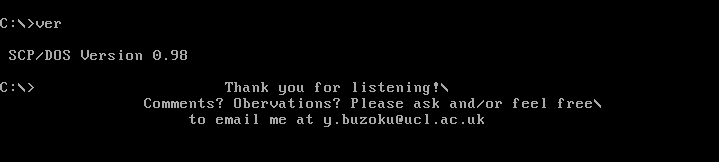
\includegraphics[width=\textwidth]{dosthanks2.png}
	  \caption{Thank you from DOS!\,:D}
	\end{center}
  \end{figure}
\end{frame}
%%%%%%%%%%%%%%%%%%%%%%%%%%%%%%%%%%%%%%%%%%%%%%%%%%%%%%%%
\begin{frame}[allowframebreaks]
	\frametitle{References}
	\nocite{*}
	\bibliographystyle{amsalpha}
	\bibliography{./refs/refs.bib}
\end{frame}
%%%%%%%%%%%%%%%%%%%%%%%%%%%%%%%%%%%%%%%%%%%%%%%%%%%%%%%%
\end{document}
